
\documentclass[paper=a4]{article}

\usepackage[left=4.5cm, right=4.5cm, top=2cm, bottom=2.8cm
  %,showframe% <- only to show the page layout
]{geometry}

\addtolength{\parskip}{\baselineskip} 
\parindent 0pt

\usepackage{graphicx}
\usepackage{config}

\usepackage{titling}
\setlength{\droptitle}{-7em}

\usepackage{authblk}

\renewcommand\Affilfont{\fontsize{9}{10.8}\itshape}

\title{Non-random network connectivity comes in pairs}
\date{}
\author[1,2]{Felix Z.~Hoffmann}
\author[1]{Jochen Triesch}

\affil[1]{Frankfurt Institute for Advanced Studies (FIAS), Johann Wolfgang Goethe University, Frankfurt am Main, Germany}
\affil[2]{International Max Planck Research School for Neural Circuits, Max Planck Institute for Brain Research, Frankfurt am Main, Germany}

\renewcommand\Authands{ and }



\begin{document}

\pagenumbering{gobble}

\maketitle

%% \begin{center}
%% {\Large{\textbf{ Non-random network connectivity comes in pairs }}}

%% %(connection probablities that are symmetric in pairs)
%% \end{center}
%% \centerline{}
%% \centerline{Felix Z.~Hoffmann, Jochen Triesch}
\vspace{-1.6cm}
Overrepresentation of bidirectional connections in local cortical networks has been repeatedly reported \cite{Markram1997,Song2005,Perin2011} and is in the focus of the ongoing discussion of non-random connectivity in local circuits in the brain. However, the exact relation between the relative occurrence of reciprocally connected pairs and structured connectivity has not been explained.

In this theoretical work we show that in a network in which connection probabilities are symmetric in pairs, $P_{ij} = P_{ji}$, the occurrence of bidirectional connections and non-random structures are inherently linked; an overabundance of reciprocal pairs emerges necessarily when the network structure deviates from a random network in any form. For this we consider a random graph model in which each edge has a separate probability $P_{ij}$ to exist and show that when these probabilities are symmetric in pairs, the expectation for bidirectional connections $\mathbf{E}(P_{ij}^2)$ is minimal for an Erd\H{o}s-R\'{e}nyi network \cite{Jensen1906, Gilbert1959}.

For two distributions of connection probabilities, the discrete two-point distribution and the continuous gamma distribution, we quantify how deviations from an Erd\H{o}s-R\'{e}nyi network structure increase reciprocity in the network. Representing different network connectivity principles, such as functionally specific connectivity and distance-dependent connectivity, both the discrete and continuous distribution can easily be tuned to account for a significant overrepresentation of bidirectional connections.

\vspace{0.8cm}
\begin{figure}[h!]
  \centering
  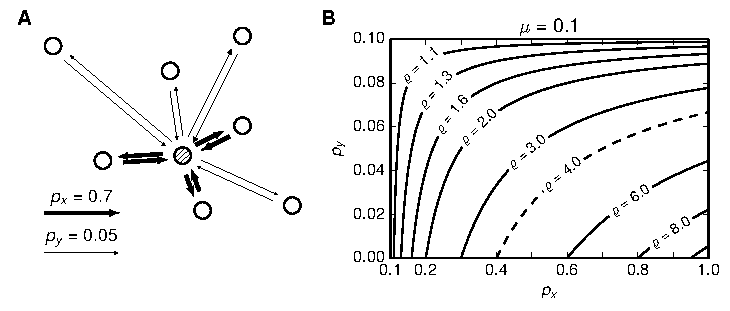
\includegraphics[width=\textwidth]{%
    img/two_point_full_pxpy.pdf} %
  \caption{Relative overrepresentation $\varrho$ of bidirectional connections in networks with a fraction of pairs connected with a high probability $p_x$ and the rest connected with a low probability $p_y$ (two-point distribution). Values of $\varrho$ as reported in [2] are easily obtained (dashed line).}
\end{figure}

\clearpage

\section*{Acknowledgements}

\section*{Topic}

Neurons, networks, dynamical systems


\printbibliography

\end{document}
